\documentclass[12pt]{article}
\usepackage{tikz}
\usepackage{amssymb}
\usepackage{amsmath}
\usepackage{breqn}

\usetikzlibrary{automata, positioning, arrows}

\title{SE 3310 Theoretical Foundations of Software Engineering Assignment 2}
\author{Marcus Tuen Muk}
\date{February 09 2023}


\begin{document}

    \begin{titlepage}
        \clearpage\maketitle
        \thispagestyle{empty}
    \end{titlepage}

    \section{Identify the regular languages}
        \textbf{Notation Preliminaries}
        \begin{itemize}
            \item The notation 0^+ means "one or more copies of 0."
            \item The notation '+' means 'or.' So (0+1) means "0 or 1"
            \item The Kleene star notation '*' repeats the item zero or more times. 
        \end{itemize}
        

        \subsection{Draw an NFA that recognizes the language generated by the following regular expression:}
            \[10^*(01)^++0(00+11)^*\]

            \begin{figure}[ht]
                \centering
                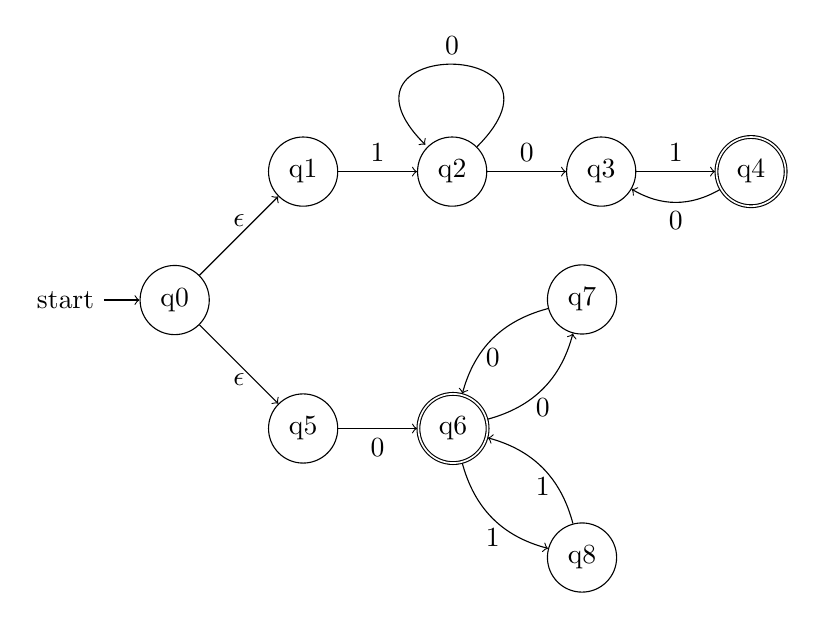
\begin{tikzpicture}
                    \node[state, initial] (q0) {q0};
                    \node[state, above right = of q0] (q1) {q1};
                    \node[state, right = of q1] (q2) {q2};
                    \node[state, right = of q2] (q3) {q3};
                    \node[state, accepting, right = of q3] (q4) {q4};
                    \node[state, below right =  of q0] (q5) {q5};
                    \node[state, accepting, right = of q5] (q6) {q6};
                    \node[state, above right = of q6] (q7) {q7}; 
                    \node[state, below right = of q6] (q8) {q8};                      

                    \draw   (q0) edge[->, right] node[above]{$\epsilon$} (q1)
                            (q1) edge[->, right] node[above]{1} (q2)
                            (q2) edge[->, loop, above] node[above]{0} (q2)
                            (q2) edge[->, right] node[above]{0} (q3)
                            (q3) edge[->, right] node[above]{1} (q4)
                            (q4) edge[->, bend left] node[below]{0} (q3)

                            (q0) edge[->, right] node[below]{$\epsilon$} (q5)
                            (q5) edge[->, right] node[below]{0} (q6)
                            (q6) edge[->, bend right] node[below]{0} (q7)
                            (q7) edge[->, bend right] node[below]{0} (q6)
                            (q6) edge[->, bend right] node[below]{1} (q8)
                            (q8) edge[->, bend right] node[below]{1} (q6);
                \end{tikzpicture} 
            \end{figure}
            
    \pagebreak
               
        \subsection{Draw an NFA that recognizes the language generated by the following regular expression:}
            \[1^*00^*+(00+1)^*\]

            \begin{figure}[ht]
                \centering
                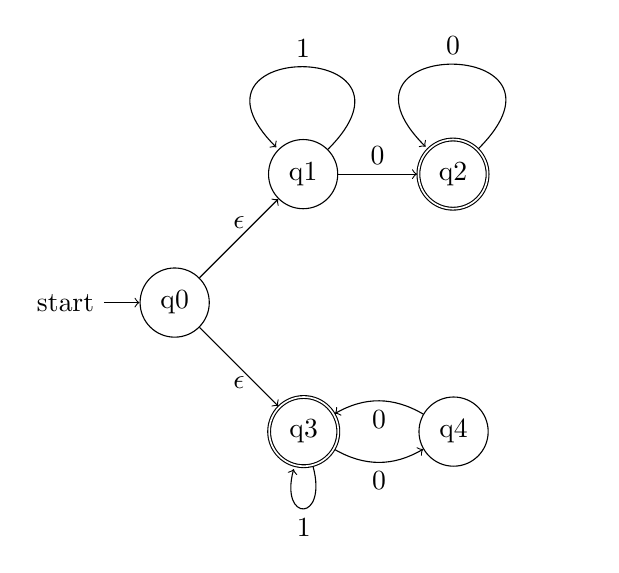
\begin{tikzpicture}
                    \node[state, initial] (q0) {q0};
                    \node[state, above right = of q0] (q1) {q1};
                    \node[state, accepting, right = of q1] (q2) {q2};
                    \node[state, accepting, below right =  of q0] (q3) {q3};
                    \node[state, right = of q3] (q4) {q4};
                         

                    \draw   (q0) edge[->, right] node[above]{$\epsilon$} (q1)
                            (q1) edge[->, loop, above] node[above]{1} (q1)
                            (q1) edge[->, right] node[above]{0} (q2)
                            (q2) edge[->, loop, above] node[above]{0} (q2)

                            (q0) edge[->, right] node[below]{$\epsilon$} (q3)
                            (q3) edge[->, bend right] node[below]{0} (q4)
                            (q4) edge[->, bend right] node[below]{0} (q3)
                            (q3) edge[->, loop below] node[below]{1} (q3);
                \end{tikzpicture} 
            \end{figure}

        \pagebreak
               
    \subsection{Describe the language generated by the following regular expression. Assume strings in this language are interpreted as binary integers}
            \[(1+0)^*00^++(100+1100)^*\]

            This expressions generates a language that produces a binary integer that is divisable by 4.
            In the first half of the expression (\((1+0)^*00^+\)) produces a binary integer
            that is divisable by 4. The lowest binary integer produced is either 0 or 4, thus excluding
            the numbers that are not divisable by 4.
            \\ \\
            Similarly, the second half of the expression (\((100+1100)^*\) produces a binary integer
            that is divisable by 4. The woest binary integer produced is either 4 or 12.
            Though this part of the expression is redundant as it is essentially covered
            by the first part of the expression.

    \pagebreak

    \section{Pumping Lemma}
    The following proofs should be made by contradiction, i.e., 
    by assuming the language is regular and working toward a contradiction using the pumping lemma.
    \\ \\
    There is no specific format or style guide for presenting 
    proofs but it should follow the methodology and process as presented in 
    the lecture/tutorial/textbook.
        
    \pagebreak

    \subsection{Use the Pumping Lemma to prove the following language is not regular:}
        \[L_a = \{1^n2^n3^n:n>0\}\]
        
        Let $L_a$ be regular

        Let $p$ be the pumping length.

        Let $s = 1^p2^p3^p$ and $s \in L_a$ as it follows the structor of the 
        given language.
        
        The cardinality of s, $|s| = 3p$, is greater than $p$.
        
        Based on these assumptions, we can now continue with the Pumping Lemma
        by splitting $s$ into 3 parts: \\ Let $s = xyz$.

        Assuming $L_a$ is regular, then $s_i = xy^iz : i \geq 0$. 
        
        Assume $y \in 1^p$, then pumping $y$ will result in the following:

        \begin{center}
            Let $s^'=xy^2z$.

            Then based on previously established assumptions,
            \[s^' = xyyz\]
            \[= 1^{p + |y|} 2^p3^p\]
            $|y| > 0$ by definition, thus making $s^'$ will have more 1s than 2s or 3s. 
            Thus $s^' \notin L_a$ since $L_a$ states that the number of 1s, 2s and 3s should be equal. 
        \end{center}

        Therefore, $L_a$ can only be regular if $y$ contains something more than just 1s.

        Now looking at the 3rd point in the pumping lemma definition:

        \begin{center}
            $|xy| \leq p$

            Since $s$ begins with $p$ number of 1s, it would mean that $xy$ must be only within
            the 1s part of $s$. Therefore $y$ must only contain 1s, contradicting the previous assumption.
        \end{center}

        Therefore, there is no way to divid $s$ into 3 parts, such 
        $xyz \in L_a$. Also, $s^' = xy^2z \notin L_a$ which goes against 
        pumping lemma, \textbf{thus making $L_a$ not regular.}
        
    \pagebreak

    \subsection{Use the Pumping Lemma to prove the following language is not regular:}
        \[L_b = \{a^p : p \ is \ prime, \ p \in \{2,3,5,7,11,...\}\}\]

        \textbf{Assumptions:}
        \begin{center}
            Let $L_b$ be regular.

            Let $p$ be the pumping length.

            Let $s = a^k$, where k is a prime greater than $p$.

            $|s| = k > p$ by definition since $k$ is greater than $p$. Also, 
            $s \in L_b$ since $k$ is prime.
        \end{center}

        Based on these assumptions, we can use pumping lemma:

        \begin{center}
            Let $s = xyz$ and $s_i = xy^iz: i \geq 0$

            To prove that this is not regular, we just need to find the case 
            where $s_i \in L_b$.

            So let $s^' = xy^{k+1}z$
            
            To prove that $k+1$ is not prime:
            
            Since $|s| = |xyz| = k$, then
            
            $|s^'| = |xy^{k+1}z|$

            $= |xyz| + |y^k|$

            $= k + k|y|$
            
            $= k(1+|y|)$
        \end{center}

        Let $m = 1+|y|$ and by definition $|y| > 0|$. So, 
        $m > 1$. Since $|s^'| = km$, it produces a prime number, $k$ and 
        an interger, $m$, $km$ is not a prime since a prime is the product of 1 and itself.
        Since $m > 1$, $km$ is the product of a prime and an integer greater than 1.

        \medskip

        Since we can't split $s$ into 3 parts, such $xy^iz \in L_b$, and 
        that $s^' \notin L_b$. \textbf{Therefore, $L_b$ is not regular.}



\end{document}